\chapter{Position Sizing}

LET'S COME BACK TO SERGEI'S THREE QUESTIONS FROM CHAPTER seven. First, how much do you like this trade? This is the forecast for each instrument. Secondly, how much can you afford to lose? You should know how many chips of trading capital you're willing to put down on the hypothetical casino baize depending on your desired target volatility. So far, so good. But how many shares, bonds, spread bet points or futures contracts should you actually buy or sell? What does a combined forecast of -6 and a £1,000,000 annualised cash target volatility mean in practice if you're trading crude oil futures in New York? To answer this we need to come back to Sergei's third question: how risky is your trade?

Once you know this you can move from the abstract world of forecasts and trading rules to deciding the size of actual positions in real financial instruments.

\section*{Chapter overview}
\phantomsection
\addcontentsline{toc}{section}{Chapter overview}

\begin{tabularx}{\textwidth}{@{}p{0.30\textwidth}Y@{}}
\textbf{How risky is it?} & If you own one unit of an instrument how much risk does that expose you to? \\
\textbf{Volatility target and position risk} & What is the relationship between your cash volatility target and the risk of each instrument? \\
\textbf{From forecast to position} & Given how confident you are in your forecasts, the cash volatility target you have and the position risk, what size position should you be holding? \\
\end{tabularx}

\section*{How risky is it?}
\phantomsection
\addcontentsline{toc}{section}{How risky is it?}

What is the expected risk of holding an instrument?\footnote{Notice we're dealing here with expected, predictable risk, as discussed on page 39.} If you own one Apple share or one crude oil futures contract, how much danger are you exposed to?

\subsection*{Position block and block value}

Let's start by asking a philosophical question. What exactly is ‘one' of an instrument? I define this as the instrument block. If ‘one' of an instrument goes up in price by 1\% how much do you gain or lose? This is the block value. These definitions will seem trivial to equity investors. ‘One' Apple share is exactly that -- one Apple share. If a share has a price of \$400 it will cost exactly \$400 to buy one block. If the price goes up by 1\% from \$400 to \$404 then you will gain \$4. Apple shares, and most other equities, have a natural instrument block of one share and a block value of 1\% of the price. Sometimes though to reduce costs you'll trade in larger blocks, usually of 100 shares. In this case the block value will be 100 × 1\% × share price, which is equal to the cost of one share. But life isn't always that simple. For example you can use a UK financial spread betting firm to bet on the FTSE falling at £10 a point. If the FTSE rises 1\% from 6500 to 6565 you would lose £650. Here the block value is ten times 1\% of the price. Futures contracts also have non-trivial block values. WTI crude oil futures on NYMEX are quoted in dollars per barrel. But each futures contract is for 1000 barrels. This means

a 1\% move up in price from \$75 to \$75.75 will net you \$750 on a long position of one contract, giving a block value of \$750. A Eurodollar future represents the cost of nominally borrowing \$1 million for three months and is priced at 100 minus the annual interest rate. If the price rises by 1\% from 98.00 to 98.98 then the rate of interest payable has fallen from 2\% to 1.02\%. Because three months is a quarter of a year you will have saved \$1 million × 0.98\% × 0.25 = \$2,450 in interest on your loan. The block value is \$2,450.110

\subsection*{Price volatility}

We've established that a 1\% fall in quoted price will cause a certain degree of pain, equal to the block value, for each instrument block of an instrument that you're long. But how likely is a 1\% fall in price? Equity prices can easily change by 1\% or more in minutes, but a two-year bond might not see a 1\% move over several months. How should you take these different levels of risk into account? This is another job for volatility standardisation. You need to calculate an expected standard deviation of daily instrument percentage returns, which I'm going to define as the price volatility of an instrument. So for example the price volatility of an average equity is around 1\%, whereas as I write this the German two-year Schatz bond future has a daily standard deviation of just 0.02\%.

CONCEPT: MEASURING RECENT STANDARD DEVIATION Remember that my standard definition of predictable risk (from page 39) is the expected daily standard deviation of prices. One of the simplest ways to estimate future volatility is to use a measure of recent standard deviation. This works surprisingly well because volatility tends to persist; if the market has been crazy over the last few weeks it will probably continue to be crazy for a few more weeks. I recommend using one of three methods to calculate recent standard deviation. The first method is to eyeball the chart. If you look at figure 22 you can see that the average daily change in crude oil futures over the last month of the chart is around \$1.0 a day, or 1.33\% of the final price of \$75. This method is fine for semi-automatic traders who will probably be staring at charts anyway, but I don't recommend it for others. The second method is to calculate the precise standard deviation of price changes over a moving window of time -- the volatility look-back period. You can use a

short window like ten business days (around two weeks), or a longer one such as 100 days. As the upper panel of figure 23 shows, shorter windows mean your volatility estimate is noisy, which as you'll see in chapter twelve will mean higher trading costs, but reacts very quickly to changes. The slower estimate is smoother, however it takes longer to adjust to new volatility environments. It's not obvious which look-back would be best. In my research I found almost no difference in performance before costs for lookback periods from a few days up to six months in length.111 Rather than risk overfitting I decided on a default look-back of 25 business days, or five weeks. This corresponds to the most popular value used across the industry, for example by the RiskMetrics (TM) system.112 I'll discuss in chapter twelve, ‘Speed and Size', when and why you'd use a longer look-back for instruments that are expensive to trade. The lower panel of figure 23 shows the volatility estimation using a 25 day lookback. It also shows the estimate coming from my third method, which is to use an exponential weighted moving average (EWMA) of standard deviation. This gives a smoother measure than a simple moving average that still reacts quickly to significant changes in the state of the market. I've chosen the default look-back for this as 36 days, which is equivalent to a 25 day window for a simple moving average.\footnote{The two measures have the same half-life when using a 25 day look-back for the simple moving average, and 36 days for exponentially weighted.} Details of how to calculate volatility with both kinds of moving average are shown in appendix D on page 298. Using recent price volatility is generally a good way to get the right risk adjusted position size. However it would be a disaster if you were using this method to trade Credit Default Swaps in early 2007, the front of the Eurodollar futures curve at any time in the US zero interest rate period, or for that matter Swiss franc FX in early January 2015. During all of these periods there was really low price volatility. If volatility is low then you would buy large numbers of instrument blocks, since each block has very little expected risk. But after periods of calm markets have a nasty habit of becoming crazy overnight, leaving you with dangerously large positions. As I've already mentioned in earlier chapters, holding very low volatility assets is generally a bad idea, and this is yet another reason to avoid them.

\begin{enumerate}
  \item Much slower than six months and performance gets steadily worse.
  \item As of 2015 RiskMetrics (TM) is owned by MSCI but it was originally developed by JP Morgan. It uses an exponentially weighted moving average whose half-life is equivalent to that of a 25 day simple moving average.
\end{enumerate}

\begin{figure}[htbp]
  \centering
  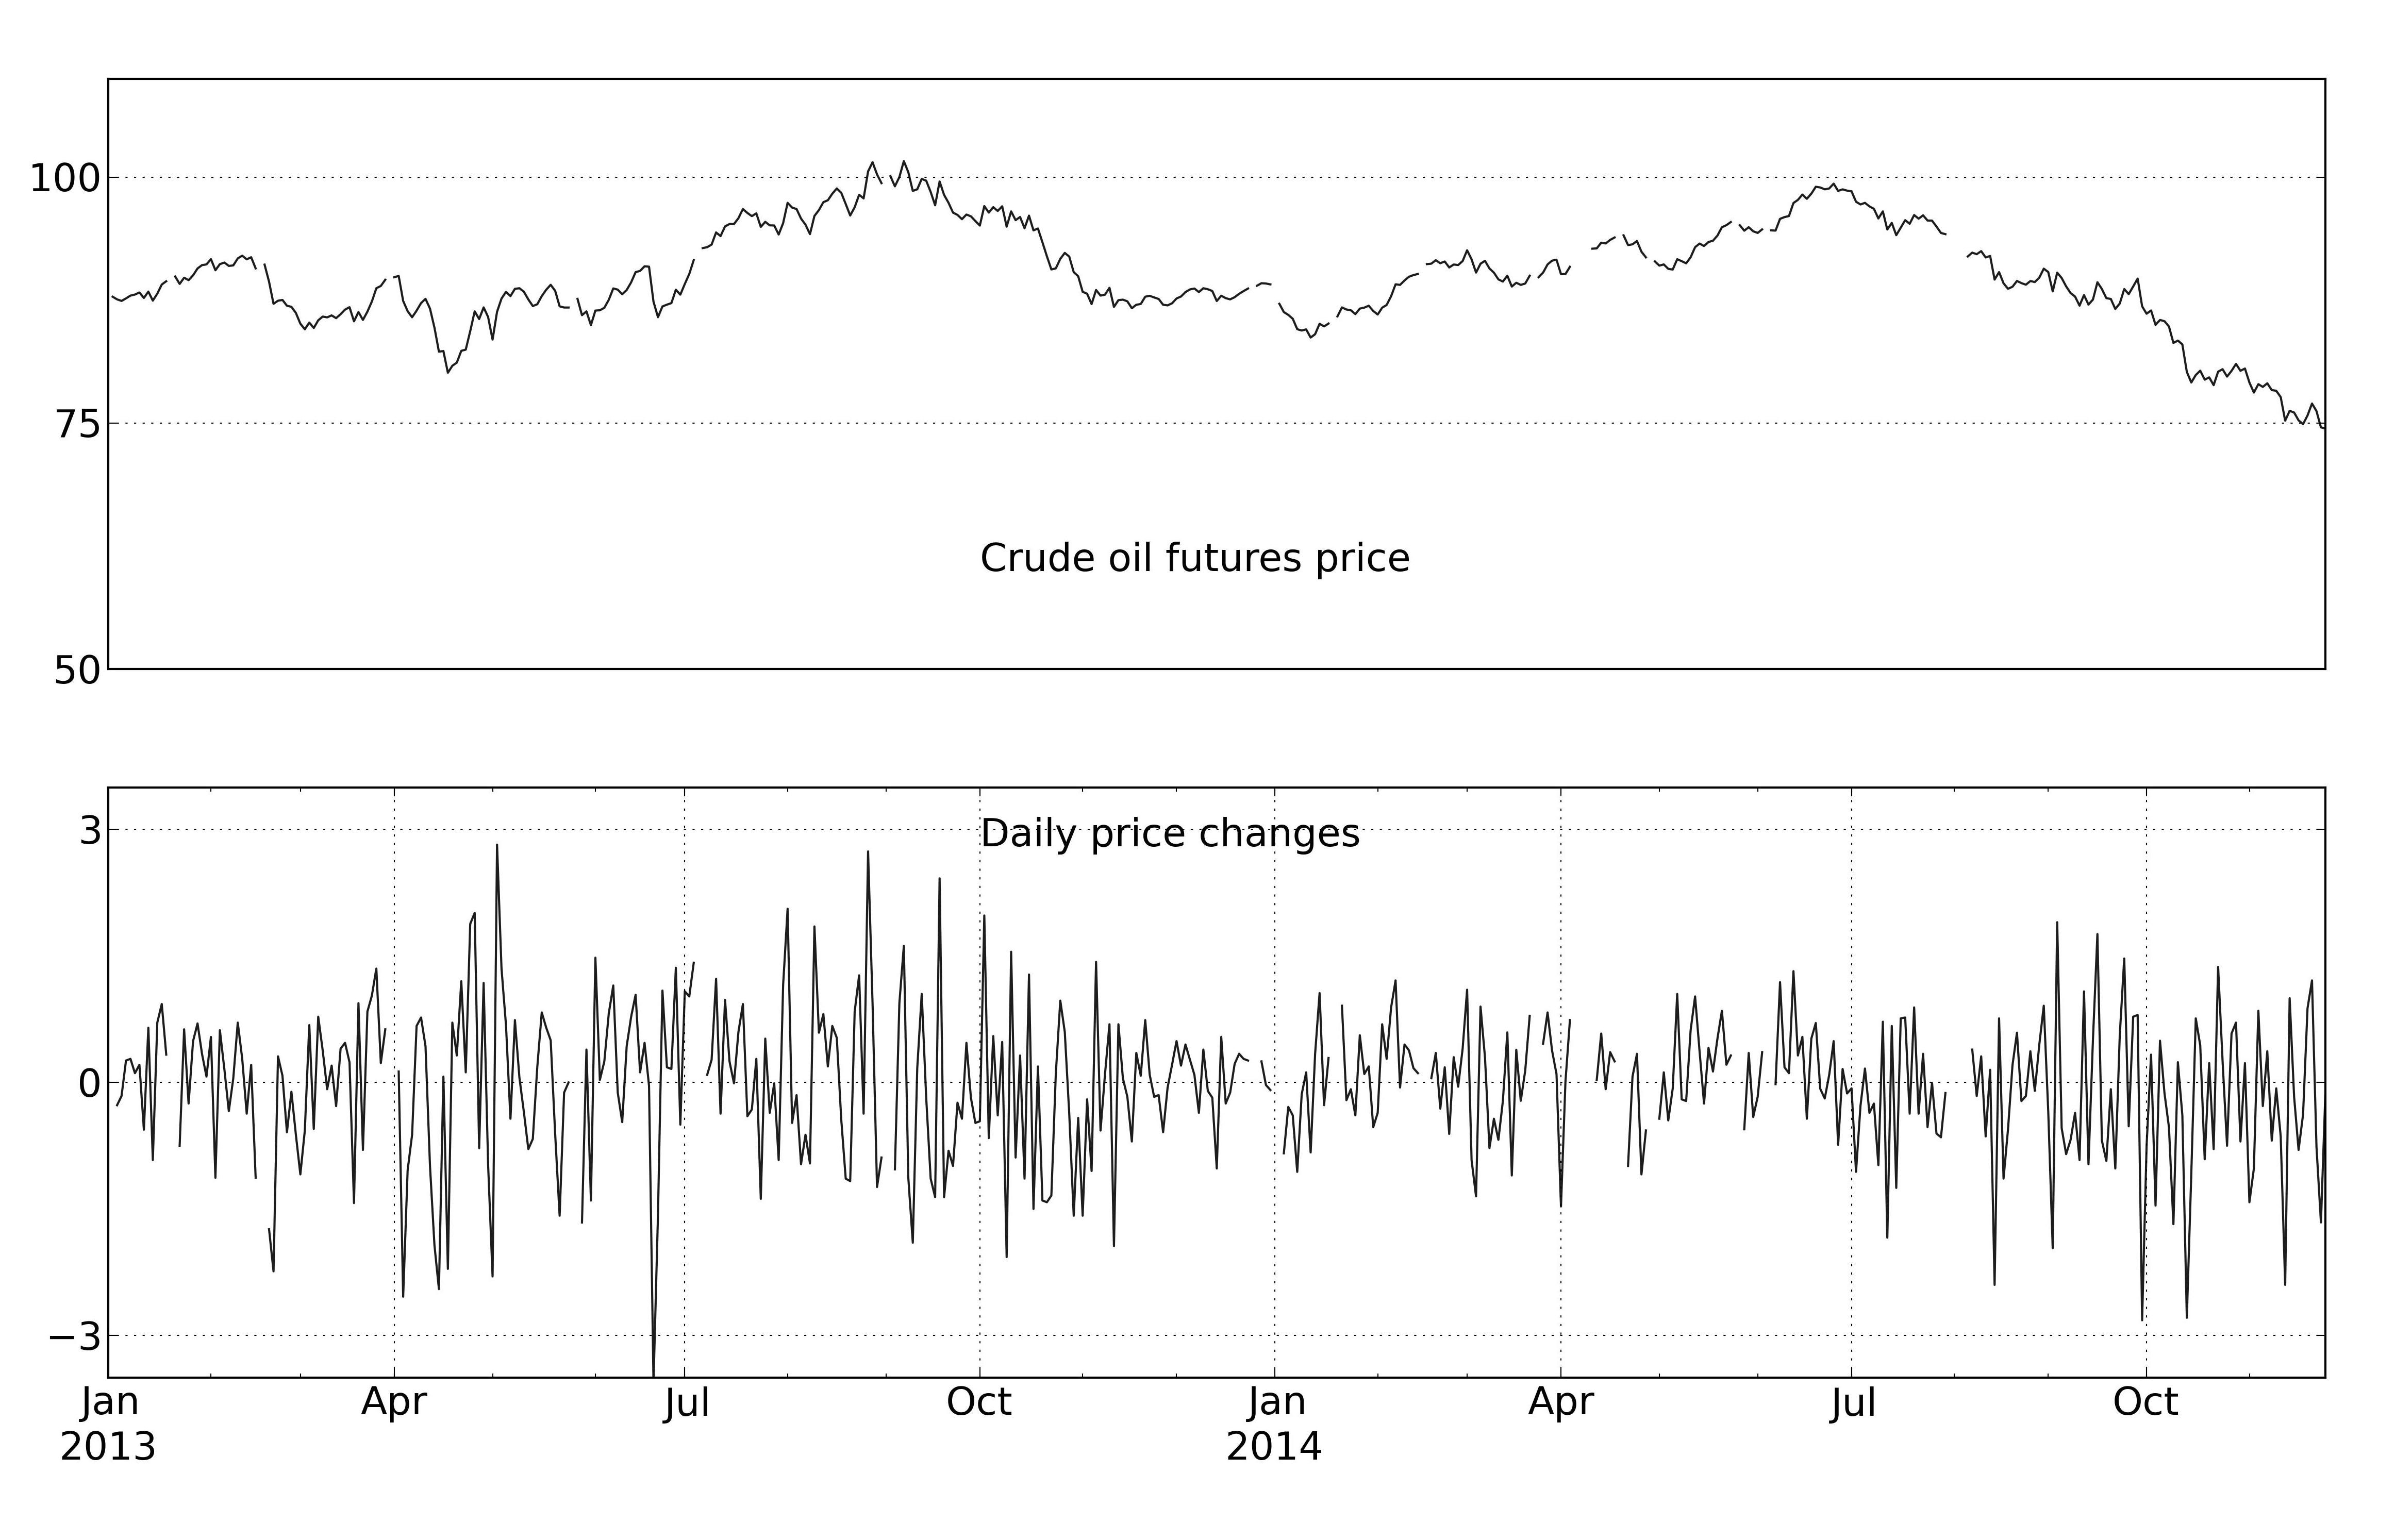
\includegraphics[width=\textwidth]{figures/raw/img-022.png}
  \caption{PRICE AND DAILY CHANGES IN CRUDE OIL FUTURES}
\end{figure}

\begin{figure}[htbp]
  \centering
  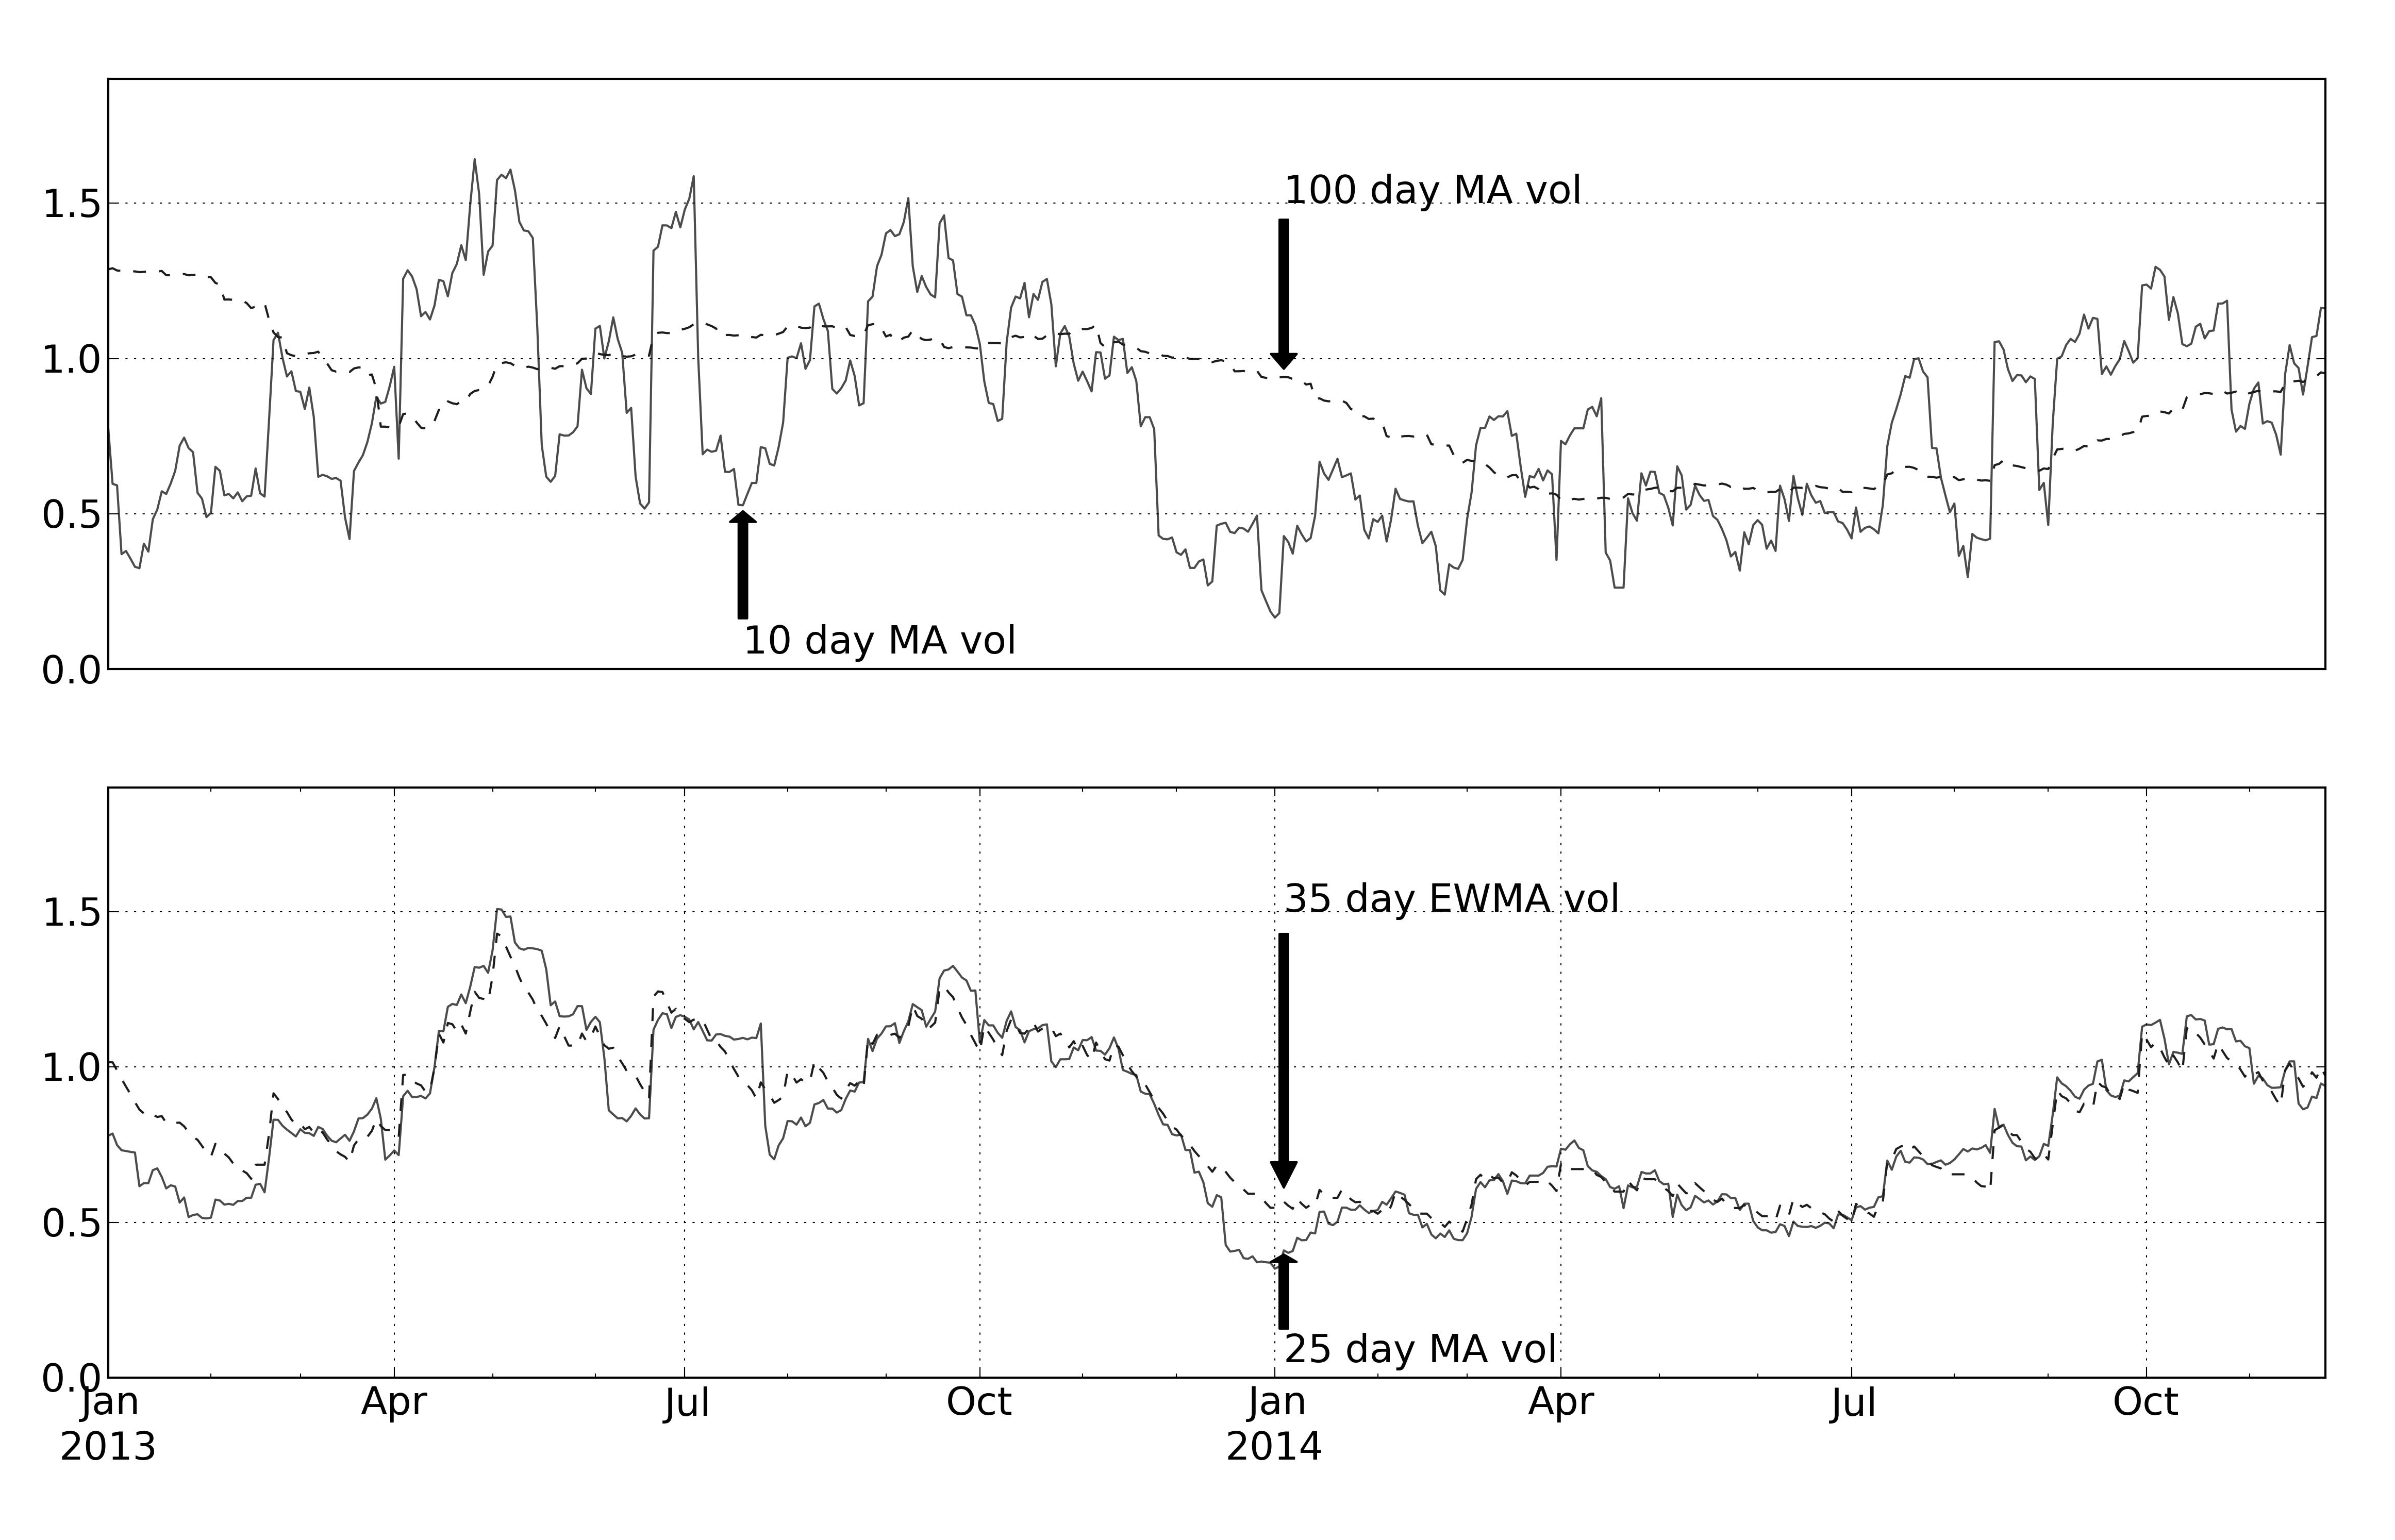
\includegraphics[width=\textwidth]{figures/raw/img-023.png}
  \caption{MEASURING CRUDE OIL PRICE VOLATILITY USING SIMPLE MOVING AVERAGE (MA) AND EXPONENTIALLY WEIGHTED (EWMA) STANDARD DEVIATIONS WITH VARIOUS LOOK- BACKS, IN DAYS}
\end{figure}

Returning to the example I opened the chapter with, if you use the bottom panel of figure 23 the price volatility of crude oil futures here is around \$1 per day, which is 1.33\% of the final price shown (\$75).

\subsection*{Instrument currency volatility}

If one oil futures contract has a block value of \$750, and a price volatility of 1.333\%, then what is the risk of owning one contract? This is the instrument currency volatility; it's the expected standard deviation of daily returns from owning one instrument block in the currency of the instrument. For oil futures you'd expect on any given day to see a price move of around 1.33\% and since each 1\% price move will cost you \$750, your daily profit or loss will average around 1.33 × \$750 = \$997.50. So the instrument currency volatility for WTI crude oil futures is \$997.50. This value shouldn't be rounded. In general instrument currency volatility is equal to the block value multiplied by the price volatility. It will be in the same currency in which the block value is measured.

\subsection*{What's that in real money?}

This is all fine if you are a US investor trading crude oil futures, a Brit trading UK equities, or a Euro area investor buying German bonds. However many investors and traders will want to buy and sell in currencies that are different from their trading capital. The instrument currency volatility isn't good enough. Instead you need to know the volatility of the instrument value in the currency of your account, which will be the same currency as your cash volatility target. I call this the instrument value volatility. The instrument currency volatility needs to be converted to an instrument value volatility using an appropriate exchange rate. The exchange rate will have the currency of the instrument as the numerator, and the account value currency as the denominator. As an example for a UK investor with a GBP account, the instrument currency volatility of a crude oil future (\$997.50) will need to be multiplied by the current USD/GBP exchange rate, to work out what those dollars are worth in British pounds. As I write this paragraph the USD/GBP rate is 0.67, giving an instrument value volatility of \$997.50 × 0.67 = £668.325. Again you shouldn't round any numbers yet. Note I'm using USD/GBP, rather than GBP/USD which is normally quoted. Be sure you are using the correct rate.

\section*{Volatility target and position risk}
\phantomsection
\addcontentsline{toc}{section}{Volatility target and position risk}

Now let's relate this back to your cash volatility target -- the risk you require and are comfortable with from your trading account. From the previous chapter on volatility targeting (page 137) your daily cash volatility target is your long-term expected daily standard deviation of returns, measured in the currency of your trading capital.

Let's refer back to the example I opened the chapter with. We had an investor with a £1,000,000 annualised cash target volatility, implying a daily target of one-sixteenth of that, £62,500.\footnote{Remember to go from annual to daily volatility you divide by the ‘square root of time'. As there are roughly 256 business days in a year, the appropriate divisor is 16.} I worked out above that the crude oil future had an instrument value volatility of £668.325 for a UK investor. This is the daily risk of owning one instrument block -- a single futures contract. How many of these blocks of crude oil should this investor hold? For now let's assume we are putting together a trading subsystem for the investor; a trading system which only has a single instrument. We'll be achieving the entire cash volatility target by having positions in just one instrument; in this case crude oil. This assumption will be relaxed in the next chapter, when we look at creating a portfolio of subsystems. We also assume that we get the required target risk by having a constant amount of expected volatility from owning a fixed long position in the asset. So we won't worry yet about the value of any forecast for the instrument. I'll consider forecasts in the next section of this chapter. For the investor in the example to get the entire required daily standard deviation of £62,500 from being long crude oil futures they need to buy £62,500, divided by the risk of one contract, £668.325, or 93.52 contracts. The value of 93.52 is a scaling factor which accounts for the difference between an instrument's natural volatility and the required volatility of the portfolio. I call it the volatility scalar. In general the volatility scalar is equal to your daily cash volatility target, divided by the instrument value volatility. You'll notice that both of these variables are in the same currency as your trading capital. Also please note that you should not round the volatility scalar to a whole number.

\section*{From forecast to position}
\phantomsection
\addcontentsline{toc}{section}{From forecast to position}

I've shown that the investor in the simple example for this chapter would need to own a long position in 93.52 crude oil futures (the volatility scalar) to realise their desired volatility target. This however ignores any forecast that the investor has made; either a combined forecast from multiple trading rules, or the single forecasts made by asset allocating investors and semi-automatic traders. At the start of the chapter I'd assumed that the forecast is -6 in the example. Clearly the investor is going to want to be short, rather than long, but by how much? To work this out you need to think about average forecasts. Over a long period of time you'll still want to be hitting your volatility target for returns, no matter what your daily forecasts are. In chapter seven (page 112) I recommended that forecasts should have a

long run average absolute value of 10. This implies that to hit your target over the long run you'd want your positions to have the same average expected variation as if you had a constant forecast of +10. Effectively then the volatility scalar gives you a position which is consistent with having a constant forecast of +10. If you're currently more optimistic with a larger positive forecast you should buy more blocks; and if you're pessimistic you should have fewer blocks, or go short if the forecast is negative. In the example above I calculated a volatility scalar of 93.52 crude oil futures contracts. This will be consistent with the long run forecast, so a forecast of +10 equates to buying 93.52 contracts (ignoring for the moment that you can't hold fractional contracts). If the forecast falls to +5 you'd only be half as confident, and want half the original position, 46.76 contracts. A forecast of -20 would mean you'd want to go short twice the original position, a sell of 187.04 blocks. The resulting quantity of blocks is the subsystem position. It's a subsystem position because, as I said earlier, we're assuming in this chapter your entire capital is invested in a subsystem trading one instrument, rather than in a complete trading system running across a number of instruments. A subsystem position is equal to the volatility scalar multiplied by the forecast, then divided by the long average of 10. So for the crude oil example with a forecast of -6, and where I've worked out the volatility scalar to be 93.52, the subsystem position will be (93.52 × -6) ÷ 10 = -56.11, implying a short of 56.11 contracts. Again you shouldn't do any rounding of non integer positions for now. If you're an asset allocating investor you've probably spotted that with a constant forecast which is always equal to +10 (from the single ‘no-rule' rule), your position will always be equal to the volatility scalar. For other traders and investors your position will depend on your forecast and on the components of the volatility scalar (your cash volatility target for your portfolio and the account value volatility of the instrument). Higher absolute forecasts, bigger account sizes, a greater appetite for risk and lower instrument price volatility will mean larger positions; and vice versa.

\section*{Summary for position sizing}
\phantomsection
\addcontentsline{toc}{section}{Summary for position sizing}

Instrument Staunch systems traders: This is the combined forecast calculated in forecast chapter eight by weighting your trading rule forecasts for an instrument and accounting for the forecast diversification multiplier. Asset allocating investors: Equal to a constant value of +10. Semi-automatic traders: Single discretionary forecast. All groups will end up with one forecast per instrument. It will have an expected average absolute value of 10 and it is limited to a range of -20 to +20.

Annualised This is the percentage volatility target multiplied by the trading capital, cash volatility from chapter nine. It's an annualised measure of expected risk from your target portfolio. It will be in units of the currency your trading capital is in.

Daily cash Annualised cash volatility target divided by ‘the square root of time'; with volatility approximately 256 business days in a year you should divide by 16. target

Price Expected daily standard deviation of instrument price changes. Watch out volatility for very low standard deviations. It will be in units of percentage of price.

Instrument This is the size you trade instruments in. For equities this would usually block be one share, though 100 shares might make sense if trading fewer is uneconomic. For futures this will be a single contract and for spread bets it is the minimum bet per point.

Block value This is how much each 1\% change in the price of a block translates into monetary value. It will be in units of instrument currency, i.e. \$ for US equities.

Instrument This is the daily standard deviation of instrument value. Equal to block value currency multiplied by the price volatility. It will be in units of instrument currency. volatility

Exchange This is the exchange rate between instrument currency (numerator) and the rate currency your trading capital is in (denominator).

Instrument Daily standard deviation of instrument value, measured in your trading value capital currency. Equal to instrument currency volatility multiplied by the volatility exchange rate. It will be in units of your account currency.

Volatility Number of position units to hold if you are investing your entire trading scalar capital in one instrument, ignoring forecasts. Equal to daily cash volatility target divided by the instrument value volatility, both in your currency. It's in units of position blocks.

Subsystem How many blocks do you need to hold given your forecast? Equal to the position instrument forecast, multiplied by volatility scalar, divided by 10. This is in units of position blocks.

\subsection*{Worked example for position sizing}

From the start of the chapter the investor in this example has an annualised £1,000,000 volatility target and is investing in WTI Crude oil futures contracts, with a forecast of -6.

Instrument -6 forecast

Annualised £1,000,000 cash volatility target

Daily cash Annualised cash volatility target divided by 16: £62,500 volatility target

Price For crude oil the bottom panel of figure 23 shows average returns of \$1 a volatility day, which with a price of \$75 equates to 1.33\%.

Instrument One futures contract block

Block value For a WTI Crude contract of 1000 barrels with price \$75 a 1\% price move will equate to \$0.75 × 1000 = \$750.

Instrument This is the block value multiplied by the price volatility. currency For crude this is \$750 × 1.33 = \$997.50 volatility

Exchange Numerator is instrument currency, USD. Denominator is account value rate currency, GBP. The USD/GBP exchange rate is currently around 0.67.

Instrument This is the instrument currency volatility multiplied by the exchange rate. value \$997.50 × 0.67 = £668.325 volatility

Volatility Daily cash volatility target divided by the instrument value volatility, both in scalar the investor's currency. £62,500 divided by £668.325 equals 93.52 contracts.

Subsystem Final combined instrument forecast, multiplied by volatility scalar, then position divided by 10. (-6 × 93.52) ÷ 10 = short 56.11 contracts (no rounding).

You can now answer all of Sergei's questions and you've finally got positions for a trading system that has a single instrument, the subsystem position. But any good trading system will have multiple assets and even semi-automatic traders normally have more than one bet on the table at a time. The next chapter examines how you can put several subsystems together into a portfolio.
